\documentclass[runningheads,a4paper,11pt]{report}
\usepackage[utf8]{inputenc}
\usepackage{algorithmic}
\usepackage{algorithm} 
\usepackage{array}
\usepackage{amsmath}
\usepackage{amsfonts}
\usepackage{amssymb}
\usepackage{amsthm}
\usepackage{caption}
\usepackage{comment} 
\usepackage{epsfig} 
\usepackage{fancyhdr}
\usepackage[T1]{fontenc}
\usepackage{geometry} 
\usepackage{graphicx}
\usepackage{hyperref} 
%\usepackage[latin1]{inputenc}
\usepackage{multicol}
\usepackage{multirow} 
\usepackage{rotating}
\usepackage{setspace}
\usepackage{subfigure}
\usepackage{url}
\usepackage{verbatim}
\usepackage{xcolor}

\geometry{a4paper,top=3cm,left=2cm,right=2cm,bottom=3cm}

\pagestyle{fancy}
\fancyhf{}
\fancyhead[LE,RO]{Project's name}
\fancyhead[RE,LO]{Team's name}
\fancyfoot[RE,LO]{ITSG 2019-2020}
\fancyfoot[LE,RO]{\thepage}

\renewcommand{\headrulewidth}{2pt}
\renewcommand{\footrulewidth}{1pt}
\renewcommand{\headrule}{\hbox to\headwidth{%
  \color{lime}\leaders\hrule height \headrulewidth\hfill}}
\renewcommand{\footrule}{\hbox to\headwidth{%
  \color{lime}\leaders\hrule height \footrulewidth\hfill}}

\hypersetup{
pdftitle={artTitle},
pdfauthor={name},
pdfkeywords={pdf, latex, tex, ps2pdf, dvipdfm, pdflatex},
bookmarksnumbered,
pdfstartview={FitH},
urlcolor=cyan,
colorlinks=true,
linkcolor=red,
citecolor=green,
}
% \pagestyle{plain}

\setcounter{secnumdepth}{3}
\setcounter{tocdepth}{3}

\linespread{1}

% \pagestyle{myheadings}

\makeindex


\begin{document}

\begin{titlepage}
\sloppy

\begin{center}
BABEȘ BOLYAI UNIVERSITY, CLUJ NAPOCA, ROMÂNIA
FACULTY OF MATHEMATICS AND COMPUTER SCIENCE
\vspace{6cm}
\Huge \textbf{}
\vspace{1cm}
\normalsize -- Autonomous assistant for medical student --
\end{center}


\vspace{5cm}

\begin{flushright}
\Large{\textbf{Team members}}\\
Crișan Camelia Daniela, Ivanov Silviu-Gabriel
\\Software-Engineering
\\group 258
\end{flushright}

\vspace{4cm}

\begin{center}
2019
\end{center}

\end{titlepage}

\pagenumbering{gobble}

\begin{abstract}
	Text of abstract. Short info about: project relevance/importance, inteligent methods used for solving, data involved in the numerical experiments; conclude by the the results obtained.
\end{abstract}


\tableofcontents

\newpage

\listoftables
\listoffigures
\listofalgorithms

\newpage

\setstretch{1.5}



\newpage

\pagenumbering{arabic}


 


\chapter{Introduction}
\label{chapter:introduction}

\section{What? Why? How?}
\label{section:what}

Motivate and abstractly describe the problem you are addressing and how you are addressing it. 
\begin{itemize}
	\item What is the (scientific) problem? 
	\item Why is it important? 
	\item What is your basic approach? 
\end{itemize}

A short discussion of how it fits into related work in the area is also desirable. Summarize the basic results and conclusions that you will present. 


\section{Paper structure and original contribution(s)}
\label{section:structure}

The research presented in this paper advances the theory, design, and implementation of several particular models. 

The main contribution of this report is to present an intelligent algorithm for solving the problem of $\ldots$.

The second contribution of this report consists of building an intuitive, easy-to-use and user
friendly software application. Our aim is to build an algorithm that will help $\ldots$.

The third contribution of this thesis consists of $\ldots$.


The present work contains $xyz$ bibliographical references and is structured in five chapters as follows.

The first chapter/section is a short introduction in $\ldots$.

The second chapter/section describes $\ldots$.

The chapter/section \ref{chapter:proposedApproach} details $\ldots$.



\chapter{Scientific Problem}
\label{section:scientificProblem}


\section{Problem definition}
\label{section:problemDefinition}

The purpose of the application is to facilitate the activity of learning the heart, of the medical students. This application will be a web application, in this way this will be accessed by every student from any device. As main functionality, the student will be able to insert an MRI (in nifty format), and as a result the student will be able to see in a 3D view the delimitation of the heart. \par
The MRI scans are gray-scale and very noisy, with a lot of organs, for the delimitation of the heart and the chambers, a specialized doctor is needed. When a medical student starts to learn about heart and its chambers, he needs a lot of research and a doctor to show him where exactly is everything. Therefore, we are trying to replace the specialized doctor by automating the whole process of segmentation.


\chapter{Related work and Usefull tools }
\label{chapter:stateOfArt}


\begin{itemize}
\item NiftyNet - deep learning library for medical imaging \url{https://niftynet.io/}
\item Mango -viewer for medical images \url{http://ric.uthscsa.edu/mango/}
\item Anaconda- open source python distribution for large-scale data processing  \\\url{https://www.anaconda.com/}
\end{itemize}


\chapter{Proposed approach}
\label{chapter:proposedApproach}

Describe your approach!

Describe in reasonable detail the algorithm you are using to address this problem. A psuedocode description of the algorithm you are using is frequently useful. Trace through a concrete example, showing how your algorithm processes this example. The example should be complex enough to illustrate all of the important aspects of the problem but simple enough to be easily understood. If possible, an intuitively meaningful example is better than one with meaningless symbols.


\chapter{Application (numerical validation)}
\label{chapter:application}


Explain the experimental methodology and the numerical results obtained with your approach and the state of art approache(s).

Try to perform a comparison of several approaches.

Statistical validation of the results.

\renewcommand{\labelitemii}{$\circ$}
\renewcommand{\labelitemiii}{\scalebox{0.5}{$\blacksquare$}}
\section{Methodology}
\label{section:methodology}

\begin{itemize}
    \item Fully convolutional neuronal network
    \item NiftyNet network
     \begin{figure}[htbp]
	    \centerline{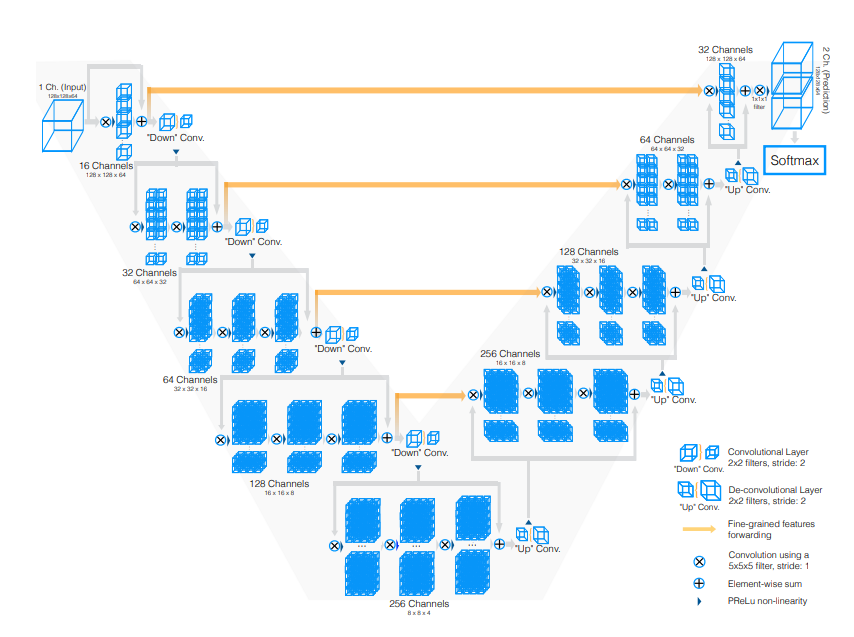
\includegraphics{Images/NiftyArch.png}}  
	    \caption{Nifty architecture}
	\label{NiftyArch}
    \end{figure}
    \item The network is composed by two paths the compression path and the decompression path until original size is reached
    \item Convolutions are performed in each stage using volumetric kernels with 5x5x5 voxels
    \item The algorithm was trained with CUDA on the GPU
    \item Creating an anaconda environment for development
    \item Processing \& Training:
    \begin{itemize}
        \item Input is a set of nifty images, format via NiBabel library
        \item The system, sets the CUDA visible devices, and queue length for network
        \item Network is the intelligent module of the application
        \item Loss function type is Dice
        \item Data-set is 80\% training and 20\% validation
        \item Seeking for 3 classes 
        \item Data augmentation:
        \begin{itemize}
            \item A random angle is computed and applied for each axis
            \item Flipping axes
            \item Random scaling on volumes
        \end{itemize}
    \end{itemize}
    \item TensorBoard used for loss graphs
    \item Loss example:
    

    \begin{figure}[htbp]
	    \centerline{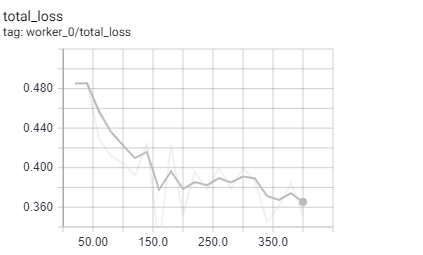
\includegraphics{Images/Loss.png}}  
	    \caption{Loss graphic after 350 iterations}
	\label{loss350}
    \end{figure}

\end{itemize}

\section{Data}
\label{section:data}

Describe the used data.

\section{Results}
\label{section:results}

Present the quantitative results of your experiments. Graphical data presentation such as graphs and histograms are frequently better than tables. What are the basic differences revealed in the data. Are they statistically significant?

\section{Discussion}
\label{section:discussion}

\begin{itemize}
	\item Is your hypothesis supported? 
	\item What conclusions do the results support about the strengths and weaknesses of your method compared to other methods? 
	\item How can the results be explained in terms of the underlying properties of the algorithm and/or the data. 
\end{itemize}



\chapter{Conclusion and future work}
\label{chapter:concl}

Try to emphasise the strengths and the weaknesses of your approach.
What are the major shortcomings of your current method? For each shortcoming, propose additions or enhancements that would help overcome it. 

Briefly summarize the important results and conclusions presented in the paper. 

\begin{itemize}
	\item What are the most important points illustrated by your work? 
	\item How will your results improve future research and applications in the area? 
\end{itemize}


\bibliographystyle{plain}
\bibliography{BibAll}

\end{document}